% ******************************* PhD Thesis Template **************************
% Please have a look at the README.md file for info on how to use the template

% For printing:
\documentclass[a4paper,12pt,times,numbered,print,twoside,sips]{Config/PhDThesisPSnPDF}

% For online pdf:
% \documentclass[a4paper,12pt,times,numbered,oneside,custommargin,sips]{PhDThesisPSnPDF}

% ******************************************************************************
% ******************************* Class Options ********************************
% *********************** See README for more details **************************
% ******************************************************************************

% `a4paper' or `a5paper': A4 pages are used for a USYD AMME thesis.
%
% `11pt' or `12pt'(default): 12pt font should be used for an AMME thesis.
%
% `oneside' or `twoside'(default): Printing double side (twoside) or single
% side.
%
% `print': Use `print' for print version with appropriate margins and page
% layout. Leaving the options field blank will activate Online version.
%
% `index': For index at the end of the thesis (not needed for AMME thesis)
%
% `sips': Add this option for a SIPS thesis, including an executive summary
% and practical experience reporting appendix chapter.
%
% `draftclassic': For draft mode without loading any images (same as draft in book)
%
% `draft': Special draft mode with line numbers, images, and water mark with
% timestamp and custom text. Position of the text can also be modified.
%
% `abstract': To generate only the title page and abstract page with
% dissertation title and name, to submit to the Student Registry
%
% `chapter`: This option enables only the specified chapter and it's references
%  Useful for review and corrections.
%
% ************************* Custom Page Margins ********************************
%
% `custommargin`: Use `custommargin' in options to activate custom page margins,
% which can be defined in the preamble.tex. Custom margin will override
% print/online margin setup. Note that the defaults specified for this class
% satisfy the AMME requirements (> 3cm left margin, > 2cm right margin), but
% custom margins can still be added.
%
% *********************** Choosing the Fonts in Class Options ******************
%
% `times' : Times font with math support.
%
% `fourier': Utopia Font with Fourier Math font (Font has to be installed)
%            It's a free font.
%
% `customfont': Use `customfont' option in the document class and load the
% package in the preamble.tex
%
% default or leave empty: `Latin Modern' font will be loaded.
%
% ********************** Choosing the Bibliography style ***********************
%
% `authoryear': For author-year citation eg., Krishna (2013)
%
% `numbered': (Default Option) For numbered and sorted citation e.g., [1,5,2]
%
% `custombib': Define your own bibliography style in the `preamble.tex' file.
%              `\RequirePackage[square, sort, numbers, authoryear]{natbib}'.
%              This can be also used to load biblatex instead of natbib
%              (See Preamble)
%
% **************************** Choosing the Page Style *************************
%
% `default (leave empty)': For Page Numbers in Header (Left Even, Right Odd) and
% Chapter Name in Header (Right Even) and Section Name (Left Odd). Blank Footer.
%
% `PageStyleI': Chapter Name next & Page Number on Even Side (Left Even).
% Section Name & Page Number in Header on Odd Side (Right Odd). Footer is empty.
%
% `PageStyleII': Chapter Name on Even Side (Left Even) in Header. Section Number
% and Section Name in Header on Odd Side (Right Odd). Page numbering in footer
%
% These can be customised further from line 730 in Classes\PhDThesisPSnPDF.cls

% Uncomment to change page style
\pagestyle{PageStyleII}
% ********************************** Preamble **********************************
% Preamble: Contains packages and user-defined commands and settings
%!TeX spellcheck = en_GB 
% ******************************************************************************
% ****************************** Custom Margin *********************************
% \usepackage{todonotes}
% Add `custommargin' in the document class options to use this section
% Set {innerside margin (use left or inner) / outerside margin (right or outer) / 
% topmargin / bottom margin} and other page dimensions
% Minimum specified in requirements:
\ifsetCustomMargin
  \RequirePackage[inner=35mm,outer=25mm,top=25mm,bottom=25mm,includehead,includefoot]{geometry}
%  \setFancyHdr % To apply fancy header after geometry package is loaded
\fi

% Example with original template
%\ifsetCustomMargin
%  \RequirePackage[left=37mm,right=30mm,top=35mm,bottom=30mm]{geometry}
%  \setFancyHdr % To apply fancy header after geometry package is loaded
%\fi

% Add spaces between paragraphs
\setlength{\parindent}{0pt}
\setlength{\parskip}{\baselineskip}

% Ragged bottom avoids extra whitespaces between paragraphs
\raggedbottom

% To remove the excess top spacing for enumeration, list and description
%\usepackage{enumitem}
%\setlist[enumerate,itemize,description]{topsep=0em}

% Edit spacing around titles
\RequirePackage{titlesec}
\titleformat{\chapter}[display]   
{\normalfont\huge\bfseries}{\chaptertitlename\ \thechapter}{20pt}{\Huge}   
\titlespacing*{\chapter}{0pt}{-40pt}{40pt}
\allowdisplaybreaks
\makeatletter\@openrightfalse

% Edit spacing around figures
\setlength{\abovedisplayskip}{4pt}
\setlength{\belowdisplayskip}{4pt}

% *****************************************************************************
% ******************* Fonts (like different typewriter fonts etc.)*************

% Add `customfont' in the document class option to use this section

\ifsetCustomFont
  % Set your custom font here and use `customfont' in options. Leave empty to
  % load computer modern font (default LaTeX font).
  %\RequirePackage{helvet}

  % For use with XeLaTeX
  %  \setmainfont[
  %    Path              = ./libertine/opentype/,
  %    Extension         = .otf,
  %    UprightFont = LinLibertine_R,
  %    BoldFont = LinLibertine_RZ, % Linux Libertine O Regular Semibold
  %    ItalicFont = LinLibertine_RI,
  %    BoldItalicFont = LinLibertine_RZI, % Linux Libertine O Regular Semibold Italic
  %  ]
  %  {libertine}
  %  % load font from system font
  %  \newfontfamily\libertinesystemfont{Linux Libertine O}
\fi

% ******************************************************************************
% **************************** Custom Packages *********************************

% *************************** Maths and Physics ********************************

\usepackage{mathtools}
\usepackage{amssymb}
\usepackage{amsmath}
\usepackage{amsfonts}
\usepackage{gensymb}
%\usepackage{physics}

% ************************* Algorithms and Pseudocode **************************

\usepackage{algorithm2e}
%\usepackage{algpseudocode}

% ********************Captions and Hyperreferencing / URL **********************

% Captions: This makes captions of figures use a boldfaced small font.
%\RequirePackage[small,bf]{caption}

\RequirePackage[labelsep=space,tableposition=top]{caption}
\renewcommand{\figurename}{Fig.} %to support older versions of captions.sty

\usepackage[nameinlink]{cleveref}
\crefname{app}{Appendix}{Appendices}

% \usepackage[hyphens]{url}
\usepackage{xurl}
\usepackage{hyperref}
\urlstyle{tt}

\usepackage[acronym,nonumberlist,toc]{glossaries}
% \usepackage[acronym]{glossaries}
% \makeglossaries
\makenoidxglossaries

% *************************** Graphics and figures *****************************

%\usepackage{rotating}
%\usepackage{wrapfig}

% Uncomment the following two lines to force Latex to place the figure.
% Use [H] when including graphics. Note 'H' instead of 'h'
\usepackage{float}
\restylefloat{figure}

% Subcaption package is also available in the sty folder you can use that by
% uncommenting the following line
% This is for people stuck with older versions of texlive
%\usepackage{sty/caption/subcaption}
\usepackage{subcaption}

% Support pdf as graphics
\usepackage{graphicx}

\usepackage{tikz}
\usetikzlibrary{shapes,arrows}
\usepackage{geometry}
\usepackage[templates]{genealogytree}
\usepackage{lmodern}

\usepackage{pdfpages}

% ********************************** Tables ************************************
\usepackage{booktabs} % For professional looking tables
\usepackage{multirow}

%\usepackage{multicol}
\usepackage{longtable}
%\usepackage{tabularx}


% *********************************** SI Units *********************************
\usepackage{siunitx} % use this package module for SI units


% ******************************* Line Spacing *********************************

% Choose linespacing as appropriate. Default is one-half line spacing as per the
% University guidelines

% \doublespacing
\onehalfspacing
% \singlespacing


% ************************ Formatting / Footnote *******************************

% Don't break enumeration (etc.) across pages in an ugly manner (default 10000)
%\clubpenalty=500
%\widowpenalty=500

%\usepackage[perpage]{footmisc} % Range of footnote options
%\usepackage[perpage]{footmisc} % Range of footnote options

\usepackage{amsmath}
\usepackage{amssymb}
\usepackage{enumitem}
\SetLabelAlign{myright}{\hss\llap{$#1$}}
\newlist{where}{description}{1}
\setlist[where]{labelwidth=2cm,labelsep=1em,
	leftmargin=!,align=myright,font=\normalfont}

\newcommand{\SubItem}[1]{
    {\setlength\itemindent{15pt} \item[-] #1}
}


% *****************************************************************************
% *************************** Bibliography  and References ********************

%\usepackage{cleveref} %Referencing without need to explicitly state fig /table

% Add `custombib' in the document class option to use this section
\ifuseCustomBib
   \usepackage[numbers]{natbib} % CustomBib

% If you would like to use biblatex for your reference management, as opposed to the default `natbibpackage` pass the option `custombib` in the document class. Comment out the previous line to make sure you don't load the natbib package. Uncomment the following lines and specify the location of references.bib file

%\RequirePackage[backend=biber, style=numeric-comp, citestyle=numeric, sorting=nty, natbib=true]{biblatex}
%\addbibresource{References/references} %Location of references.bib only for biblatex, Do not omit the .bib extension from the filename.

\fi

% changes the default name `Bibliography` -> `References'
\renewcommand{\bibname}{References}


% ******************************************************************************
% ************************* User Defined Commands ******************************

% *********** To change the name of Table of Contents / LOF and LOT ************

%\renewcommand{\contentsname}{My Table of Contents}
%\renewcommand{\listfigurename}{My List of Figures}
%\renewcommand{\listtablename}{My List of Tables}


% ********************** TOC depth and numbering depth *************************

% Victor changed to 3
\setcounter{secnumdepth}{3}
\setcounter{tocdepth}{3}

% ******************************* Nomenclature *********************************

% To change the name of the Nomenclature section, uncomment the following line

%\renewcommand{\nomname}{Symbols}


% ********************************* Appendix ***********************************

% The default value of both \appendixtocname and \appendixpagename is 
% `Appendices'. These names can all be changed via:

%\renewcommand{\appendixtocname}{List of appendices}
%\renewcommand{\appendixname}{Appndx}
\usepackage[titletoc]{appendix}

% *********************** Configure Draft Mode **********************************

% Uncomment to disable figures in `draft'
%\setkeys{Gin}{draft=true}  % set draft to false to enable figures in `draft'

% These options are active only during the draft mode
% Default text is "Draft"
\SetDraftText{Thesis Draft v0.1}

% Default Watermark location is top. Location (top/bottom)
%\SetDraftWMPosition{bottom}

% Draft Version - default is v1.0
\SetDraftVersion{GENERAL}

% Draft Text grayscale value (should be between 0-black and 1-white)
% Default value is 0.75
%\SetDraftGrayScale{0.8}


% ******************************** Todo Notes **********************************
% Uncomment the following lines to have todonotes.
% You can have multiple notes (uncomment \othernote line), e.g. to write notes 
% directed at your supervisor.

\makeatletter
\ifsetDraft
	\usepackage[colorinlistoftodos]{todonotes}
	\newcommand{\oftodo}[1]{\todo[size=\small,author=@OF,inline,color=orange!40]{#1}}
	\newcommand{\swtodo}[1]{\todo[size=\small,inline,author=@SW,color=red!40]{#1}}
	\newcommand{\actodo}[1]{\todo[size=\small,inline,author=@Accn,color=magenta!40]{#1}}
\else
	\newcommand{\oftodo}[1]{}
	\newcommand{\swtodo}[1]{}
	\newcommand{\actodo}[1]{}
	% \newcommand{\listoftodos}{}
	\providecommand{\@LN}[2]{}
\fi
\makeatother

% Example todo: \mynote{Hey! I have a note}

% *************************** Other custom commands ****************************

% At numbers in a long align* block
\newcommand{\numberthis}{\addtocounter{equation}{1}\tag{\theequation}}

% Custom maths symbols (examples)
%\newcommand{\Rwb}{\prescript{W}{}{R}_B}
%\newcommand{\dRwb}{\prescript{W}{}{\dot{R}}_B}
%\newcommand{\skewm}[3]{\bmqty{  0 & -#3 &  #2 \\
%							   #3 &   0 & -#1 \\
%						      -#2 &  #1 &   0 }}
%\DeclareMathOperator*{\argmin}{arg\,min}

% Victor changes
\usepackage{dirtytalk}
\newtheorem{definition}{Definition}


% Python highlighting https://tex.stackexchange.com/questions/83882/how-to-highlight-python-syntax-in-latex-listings-lstinputlistings-command

% Default fixed font does not support bold face
\DeclareFixedFont{\ttb}{T1}{txtt}{bx}{n}{10} % for bold
\DeclareFixedFont{\ttm}{T1}{txtt}{m}{n}{10}  % for normal

% Custom colors
\usepackage{color}
\definecolor{deepblue}{rgb}{0,0,0.5}
\definecolor{deepred}{rgb}{0.6,0,0}
\definecolor{deepgreen}{rgb}{0,0.5,0}
\definecolor{codegray}{rgb}{0.5,0.5,0.5}

% \usepackage{todonotes}
\usepackage{listings}

% Python style for highlighting
\newcommand\pythonstyle{\lstset{
language=Python,
basicstyle=\ttm,
morekeywords={self},              % Add keywords here
keywordstyle=\ttb\color{deepblue},
numberstyle=\tiny\color{codegray},
numbers=left,
emph={MyClass,__init__},          % Custom highlighting
emphstyle=\ttb\color{deepred},    % Custom highlighting style
stringstyle=\color{deepgreen},
frame=tb,                         % Any extra options here
showstringspaces=false,
breaklines=true,
postbreak=\mbox{\textcolor{red}{$\hookrightarrow$}\space},
commentstyle=\color{gray}\ttfamily
}}


% Python environment
\lstnewenvironment{python}[1][]
{
\pythonstyle
\lstset{#1}
}
{}

% Python for external files
\newcommand\pythonexternal[2][]{{
\pythonstyle
\lstinputlisting[#1]{#2}}}

% Python for inline
\newcommand\pythoninline[1]{{\pythonstyle\lstinline!#1!}}

% For centering large tables
\usepackage{adjustbox}

% Inline code snippet
\newcommand{\code}[1]{\texttt{#1}}
% \newcommand\myworries[1]{\textcolor{red}{#1}}
\usepackage{todonotes}
% \newacronym{zk}              {ZK}             {Zero-Knowledge}
% \newacronym{zkp}             {ZKP}            {Zero-Knowledge Proof}
% \newacronym[longplural={Zero-Knowledge Succinct Non-interactive Arguments of Knowledge}]
%            {zksnark}         {zk-SNARK}       {Zero-Knowledge Succinct Non-interactive Argument of Knowledge}

% Example usage:
% \acrlong{zkp} for long acronym
% \acrlongpl{zkp} for long acronym with plural
% \acrshort{zkp} for short acronym
% \acrshortpl{zkp} for short acronym with plural

% \newglossaryentry{VC}
% {
%   name=Verifiable Computation,
%   description={A recent branch in Computer Science relating to the verification of computation, possibly done by a malicious, dishonest actor}
% }

% Use it by:
% \gls{VC} for glossary entry
% \glspl{VC} for glossary entry with plural
% \Gls{VC} for Capitalised glossary entry
% \Glspl{VC} for Capitalised glossary entry with plural
\glsaddall

% ************************ Thesis Information & Meta-data **********************
% Thesis title and author information, reference file for biblatex
% ************************ Thesis Information & Meta-data **********************
%% The title of the thesis
\title{Investigation of The Aerodynamic Characteristics of Propeller Interactions for Mini Aerial Vehicles}
%\texorpdfstring is used for PDF metadata. Usage:
%\texorpdfstring{LaTeX_Version}{PDF Version (non-latex)} eg.,
%\texorpdfstring{$sigma$}{sigma}

%% Subtitle (Optional)
% \subtitle{Progress Report}

%% The full name of the author
\author{Jasmine Warner}

%% Department (eg. Department of Engineering, Maths, Physics)
\dept{School of Aerospace, Mechanical and Mechatronic Engineering}

%% University and Crest
\university{The University of Sydney}
\crest{
\includegraphics[height=40mm]{Config/usyd-logo.pdf}}

%% Supervisor
%% for multiple supervisors, append each supervisor with the \newline command
\supervisor{Prof. Dries Verstraete}

%% Supervisor Role (optional) - Supervisor (default) or advisor
%\supervisorrole{\textbf{Supervisors: }}
%% if no title is desired:
% \supervisorrole{}

%% Supervisor line width: required to align supervisors
\supervisorlinewidth{0.35\linewidth}

%% Advisor (optional)
%% for multiple advisors, append each advisor with the \newline command
% \advisor{Mr. Luke Higgins}
%Dr. B. Advisor}
     
%% Advisor Role (optional) - Advisor (default) or leave empty
% \advisorrole{Industry Supervisor: }
%% if no title is required
% \advisorrole{}

%% Advisor line width: required to align supervisors
% \advisorlinewidth{0.3\textwidth}


%% You can redefine the submission text:
% Default as per the University guidelines:
% ``This dissertation is submitted for the degree of''
% \renewcommand{\submissiontext}{change the default text here if needed}

%% Full title of the Degree (optional)
\degreetitle{Bachelor of Engineering Honours}
%% Submission date
% Default is set as {\monthname[\the\month]\space\the\year}
\degreedate{Jan 2022} 

%% Meta information
\subject{Engineering} \keywords{{Honours Thesis} {Engineering} {University of
Sydney}}



% ***************************** Abstract Separate ******************************
% To printout only the titlepage and the abstract with the PhD title and the
% author name for submission to the Student Registry, use the `abstract' option in
% the document class.

\ifdefineAbstract
 \pagestyle{empty}
 \includeonly{Declaration/declaration, Abstract/abstract}
\fi

% ***************************** Chapter Mode ***********************************
% The chapter mode allows user to only print particular chapters with references
% Useful option to review a particular chapter or to send it to supervisior.
% To use choose `chapter' option in the document class
% Multiple chapters can be listed.


\ifdefineChapter

 % Disable the table of contents, figures, tables, index and nomenclature
 % Comment to include any of these
 \renewcommand{\maketitle}{}
 \renewcommand{\tableofcontents}{}
 \renewcommand{\listoffigures}{}
 \renewcommand{\listoftables}{}
 % \renewcommand{\printnomencl}[1][]{}
 \renewcommand{\printthesisindex}{}
 % \renewcommand{\listoftodos}{}

 % Add chapters to include here
 \includeonly{
 	3_Chapter3/chapter3,
 }
\fi

% ***

% ******************************** Front Matter ********************************

\begin{document}

\frontmatter

\maketitle

% A dedication is often not included, uncommment and delete folder
% if not needed
%\begin{dedication} 

[Dedication]
%Dedicated to all Machine Learning researchers, developers, followers, and tinkerers the world over, whose passion will drive human advancement for decades to come.

\end{dedication}


\newpage
% Needed this to fit in my declaration.
\newgeometry{top=20mm, bottom=20mm, left=20mm, right=20mm}

\begin{declaration}
% \vspace{-3em}
I, Jasmine Warner, hereby declare that this thesis submission titled \emph{Investigation of Propeller Interactions for Mini Aerial Vehicles} is my own work and that, to the best of my knowledge and belief, it contains no material previously published or written by another person nor material which to a substantial extent has been accepted for the award of any other degree or diploma of the University or other institute of higher learning, except where due acknowledgement has been made in the text.  Specifically, the work I contributed consists of:

\vspace{-1.5em}

\begin{enumerate}
    \item Conducting the literature review
    \item Assisting in producing a 3D model of the generic micro aerial vechicle
    \item Wind tunnel testing of the generic micro aerial vechicle model
    \item Analysing data of wind tunnel results and validating collected data using VAP 3.5
    \item Writing this thesis report.
\end{enumerate}

\vspace{-1.5em}
Assistance was received from Benjamin Van Magil in the development of the MAV model.
Assistance was received from my supervisor in the areas of:

\vspace{-1em}

\begin{enumerate}
    \item Distinguishing relevant literature and indicating critical software required for this thesis
    \item Assisting in developing the final MAV model
    \item Ameliorating this thesis through constant feedback.
\end{enumerate}

\vspace{0.5cm}

\vfill
\begin{center}
    \begin{minipage}[t]{0.4\textwidth}
        \begin{flushleft}
            \rule{\textwidth}{0.5pt}\\
            Jasmine Warner\\
            \emph{Author}
            \\[1.5cm]
            \rule{\textwidth}{0.5pt}\\
            A/Prof. Dries Verstraete\\
            \emph{Supervisor}
        \end{flushleft}
    \end{minipage}
    \hspace{1cm}
    \begin{minipage}[t]{0.4\textwidth}
        \begin{flushleft}
            \rule{\textwidth}{0.5pt}\\
            Date
            \\[2.15cm]
            \rule{\textwidth}{0.5pt}
            Date
        \end{flushleft}
    \end{minipage}
\end{center}
% \vspace{1cm}


\end{declaration}
\restoregeometry

\newpage
\begin{acknowledgements}      

\end{acknowledgements}
\newpage
\cleardoublepage
\begin{abstract}

\end{abstract}

\newpage
% An additional executive summary is only needed for a SIPS theis. Can be deleted
% if not nessecary.
% TODO: Check if we need to have an abstract with title/author info for SIPS
\ifSipsThesis
	\cleardoublepage
\begin{executive}

\end{executive}

\fi

% *********************** Adding TOC and List of Figures ***********************

\listoftodos

\tableofcontents


\listoffigures

\listoftables

% \printnomencl[space] space can be set as 3em between symbol and description
%\printnomenclature[3em]

\printnomencl[6em]

% \printglossary[type=\acronymtype,title=List of abbreviations]
% \printglossary[type=main]

\printnoidxglossary[type=\acronymtype,title=List of abbreviations]
\printnoidxglossary[type=main]

%%% \newpage just to demonstrate that links are correct
\newpage


% ******************************** Main Matter *********************************
\mainmatter

\graphicspath{{./Figs/}}

\chapter{Introduction} 
\label{sec:Background}

% What is a MAV


Unmanned aerial vechicles (UAV) are used throughout various industries to conduct missions which are either dangerous, difficult or tedious for humans to perform. The development of technologies and demand for smaller aerial vechicles has lead to the development of Micro aerial vehicles (MAV) \cite{NONAMI2007}. MAV's will become evermore important for both commerical \cite{Liu2014} and millitary \cite{Chaturvedi2019} \cite{Fan2018} use as advancements are made in navigation systems, cooperative control of multiple MAV's, advanced vision systems, embedded computational systems and navigational systems.

%  MAV's do not have a standard guidelines for 
Despite the small size of MAV's there are three main categories these aircraft fit into. These are fixed wings \cite{Stanford2008} \cite{Lasek2001}, rotary wings, flapping wings\cite{Platzer2012} or a combination of these. Due to the small size and Reynolds numbers at which these aircraft operate at (typically around Re=$10^5$\cite{Huq2009}), insects and other small animals are often studied to understand the flight dynamics which occur for small flying bodies \cite{Liu2009}. The additional complexity to the design of MAV's occurs due to several factors:
\begin{itemize}
  \item Low Reynolds number flight
  \item Small physical dimensions
  \item Structural strength
  \item Reduced stall speed
  \item Low inertia
\end{itemize}

\begin{figure}[H]
  \centering
  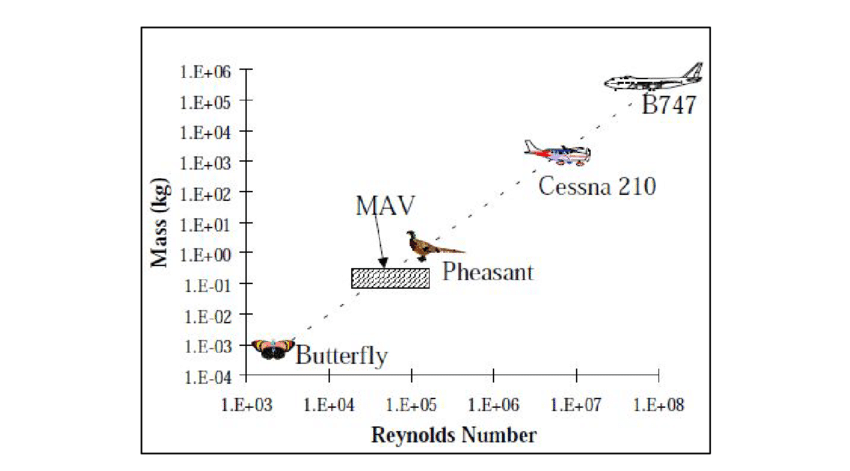
\includegraphics[width=0.8\linewidth]{images/Reynolds.png}
  \caption{Fine mesh}
  \label{fig:MAVsizes}
\end{figure}

% \\
With the increased complexity of MAV designs, there has also been increased interest in the reasearch and design of optimized MAV models \cite{Ward2017}. Current methods \todo{cite} do not produce validated, optimised and reliable designs which maximise the performance for the relevant purpose it is created for. In this area software designed to numerically optimise models based on aerodynamic properties, which are in turn mathematically determined are being used. The low Reynolds number that MAVs fly at and the influence of propeller effects on the rest of the MAV are currently unvalidated with physical wind tunnel testing. This main goal of this thesis therefore aims to fill in this gap.\\
\\
Many groups of research have \todo{cite} created software to optimize MAV's by using optimization algorthims such as generic algorthims, non-dominating sorting generic algorithms, particle swarm optimization and sequential quadratic optimisation programs. While some have accounted for low Reynolds numbers and even fewer, propeller interaction effects. None have validated these results with physical testing. These effects are expected to greatly influence the aerodynamics of MAV designs and both aspects of flight are currently unaccounted for together in physical wind tunnel testing.
\section{Background}
% Intro here

\subsection{Proliferation of MAV's in the Aerospace Landscape}
\label{subsec:ProliferationMAVs}

UAV's have existed for centuries and have been predominately used for survellience and millitary purposes \todo{cite paper}. The recent shift to the miniturization of components, systems and aerial vehicles has already influenced the military sector with several developments underway to reduce visibility of reconansance aircraft and reduce the likelihood of aircraft being detected during missions.\todo{: add examples)} What started as a small initial interest in smaller and smarter drones has resulted in exponential growth in the sector \todo{cite}. This coupled together with the growth in camera sensors and computer development, has led to the exponential growth in the capabilities of MAV seen today. Where an inital drone supported only low camera resolution with meagre flight times, today incoporates several systems such as gyrostabilisation, GPS capability with waypoint guidance, beyond the line of vision control, speeds of 70 km/h with a 30 minute flight time and a 20 megapixel camera. (DJI Phantom 4)\todo{cite Phantom}. \\

% Look at section \ref{sec:ProliferationMAVs}.

\subsection{Limitations of Current Developed MAV}
\label{subsec:Limitations}
While MAV technology is more accessible and viable to mass market than it has ever been before, there is no fully developed and validated way to optimize a MAV for a specified mission. Procedures today involve developing a CAD model of the MAV which is either then run through aerodynamic optimization software and/or tested in a wind tunnel to detemine the main characteristics of the MAV \cite{Paulson2017}. The largest drawback of which is the lack of propeller effects accounted for during wind tunnel testing. MAV model tests have been conducted with a fixed position propeller. Models are however typically tested without a free-flowing propeller, although these have been included in several aerodynamic software programs.  A lack of validation from wind tunnel testing however, means that a full understanding of the effects a propeller has on MAV's has not been conducted. Due to the small size of MAV and the large relative size of the propeller rotor disc compared to both the wing and body size it is expected that the propeller will significantly affect the stability, noise, overall endurance, performance and power consumption of a given MAV. 

\subsection{The General Micro Aerial Vechicle}
\label{subsec:GenMAV}
Today the interest, research and development of MAV's is continually increasing, however in order to focus on particular aspects or compare various designs, a "baseline" geometry is required. An example of this is the GENMAV \cite{Stewart2007}. While there are various models which have been tested to determine the main aerodyanmic properties \cite{Stewart2007}, none have completed a physical wind tunnel test while accounting for the effects of a powered propeller. Inital GENMAV aerodynamic data was determined by using the vortex-panel method \cite{Stewart2007} and did not involve wind tunnel testing. The effects of propeller induced flow has also been studied for both fixed and free-spinning propellers but currently no data is avaliable for wind tunnel tests of a powered MAV.

\subsection{Optimization Techniques and Validation}
\label{subsec:Optimization}
Many non-standard aircraft designs are evaluated using software in order to analyse aerodynamic characteristics and then optimized through a variety of typical software engineering methods such as the particle swarm method. These procedures are typically used as non-standard aircraft designs are more tedious to design and even more complex to setup and test than compared with standard aircraft designs. 

% There are many studies which have outlined methodologies for accurately determining the forces on fixed wing MAV under low Reynolds number flow streams \cite{Roberts2011} 

% \cite{Ananda2015} \cite{Roberts2011} \cite{Suhariyono2006} \cite{Zhan2012}. Propeller effects on MAV's have also been investigated


\section{Problem Statement}
\label{ProblemStatement}
MAV's are set to increase the ability to conduct a variety of missions which predominately have military or survellience objectives (todo: examples ). In the past troopers would venture on dangerous missions in order to "hopefully" gather useful information while risking their lives (todo: cite paper). Survellience was conducted initally from hot air balloons, again risking human lives. Later aircraft (mainly helicopters) would be used, costing companies large sums of money in order to survey from a birds eye view. Today drones and UAV's often conduct this work (within certain limits due to range and flight time). The next major technology jump sees the optimization and miniturization of these aircraft to produce MAV's. \\
\\
MAV's fit a niche and growing market. These aircraft are mainly used for military purposes due to the MAV's main deffering attributes; its smaller size, lower radar visibility and lower noise output.\\
\\
With MAV design becoming one of the fastest growing areas of development in the aerospace industry, there comes an increasing need to have accurate experimental data in order to validate, simulate and model the numerous MAV configurations being investigated. 

% paragraph on impact\significance of MAV
MAV's

% paragraph on current Limitations

%paragraph on lack of propeller effects


% paragraph on challenge/ main goal 
\section{Objectives}
\label{sec:Objectives}
The objectives of this thesis are as follows:

\begin{enumerate}
  \item To carry out a review of current published literature and determine areas with insufficient or no research avaliable for further development and research.
  \item To design and produce a 3D model of a generic micro aerial vechicle with interchangable empennage.
  \item To conduct wind tunnel testing of the generic micro aerial vechicle model with and without propeller effects.
  \item To analyse data of wind tunnel results and detail the affect that propeller effects have on general micro aerical vehicles.
\end{enumerate}

\section{Outline}
\label{sec:Outline}
An outline of the proposed final submission is listed below, however is subject to change.

\begin{itemize}
  \item Chapter 2: Background and literaure review of relevant topics and reasearch for this thesis
  \item Chapter 3: Proposed setup of analysis
  \item Chapter 4: Implementation
  \item Chapter 5: Results
  \item Chapter 6: Discussion
  \item Chapter 7: Conclusion
\end{itemize}



% \begin{python}[caption=Example computation]
% // Calculate the multiplication of x and y by adding x, y number of times.
% function multiply(x, y):
%   output = 0

%   for i = 0..y:
%     output = output + x

%   return output
% \end{python}


\graphicspath{{./Figs/}}

\chapter{Background} 
This section outlines the core theory and topics which are relevant for the optimization of MAV's and the effect of propeller interactions on the main wings of small MAV. MAV design is more complex than general aircraft design due to factors such as the non-linear lift distribution, low aspect ratio wings, low Reynolds number flows, structural integrity due to the small size and 


\section{Aerodynamic Parameters}
\label{sec:AerodynamicParameters}
The characteristics of an aircraft is given by a combination of the aerodynamic parameters that describe it. For MAV's this is more complex as these aircraft do not allow for the same assumptions to be made in calculations. New methods for determining the aerodyanmic parameters are currently being developed and proposed \cite{Shen2018} \cite{Roberts2011} in order to address these differences. Aerodynamic forces are cruical to the overall design of any aircraft \cite{Aero2012}. In order to determine these forces for MAV's a variety of techniques have been used such are the simple vortex lattice method \cite{Stewart2007} \cite{Hard2010}. However this method lacks the ability to predict the separetion of flow as lift is assumed to increase linearly with respect to the angle of attack \cite{Aboelezz2020}. This is not the case at low Reynolds numbers \cite{Zhang2022}. 

\cite{DeLuca2004}.
\cite{Chinwicharnam2013}

\section{Low Reynolds Number Effects }
\label{sec:LowReynolds}
Low Reynolds number compressible aerodynamics affect many different varities of aircraft. Aircraft used to survey martian terrian and MAV's are particularly influenced due to the change in atmosphere and small geometry respectively\cite{Munday2015}. This especially critical for propeller based systems as the root and tip of the mach numbers can vary significantly\cite{Munday2015}. Typically aircraft fly at high Reynolds numbers (>$10^{6}$), MAV's however generally fly between ($10^{4} and 10^{5}$) \cite{Winslow2018}.


\section{Propeller Wing Interaction}
\label{sec:Propeller Wing Interaction}
%Stability effects talked about here 

\section{MAV Optimization}
\label{sec:MAV Optimization}
Many optimization techniques exist which aim to optimize the aerodynamic design of MAV's. Algorithms such as genetic algorithms, artificial neural networks \cite{Boutemedjet2019}, 
\subsection{Wing Planform}

\subsection{Tail Planform}

\section{Non-Linear Lift Distribution}
\label{sec:Non-Linear Lift Distribution}
Early on in the study of aerodynamics, theories which were developed from the study of conventional aircraft were applied to the bodies of small flying objects and animals such as birds. Traditional aerodynamic theories provide good results and insights when steady flows move across a staionary body. They could not however explain what allows small insects and birds to fly leading to the paradox of "a bee cannot fly" \cite{bees} \cite{Roccia2016}. The issue lies in the fact that the flight of biological creatures is mainly characterized by non-linear and steady flows \cite{Roccia2016}. This non-linear lift distribution is largely caused by the low Reynolds number that these small bodies fly at and also the low aspect ratio that MAV aircraft typically have.

Wingtip vortices are particularly important and even in general aircraft lead to regulations such as spacing rules between aircraft and aerodynamic noise \cite{Qin2021}. 










\section{Stability}



\graphicspath{{./Figs/}}

\chapter{Progress} 

\label{sec:Experimental Setup}

\label{sec: Constraints and assumptions}

\label{sec: Problem Analysis}

\label{sec: Proposed solution}

\label{sec: Future Investigation}


% ********************************** Back Matter *******************************
% Backmatter should be commented out, if you are using appendices after References
%\backmatter

% ********************************** Bibliography ******************************
\begin{spacing}{1}

% To use the conventional natbib style referencing
% Bibliography style previews: http://nodonn.tipido.net/bibstyle.php
% Reference styles: http://sites.stat.psu.edu/~surajit/present/bib.htm

%\bibliographystyle{ieeetr}
%\bibliographystyle{unsrt} % Use for unsorted references
%\bibliographystyle{plainnat} % use this to have URLs listed in References
\bibliographystyle{Config/OscarBibStyle} % Oscar's custom job
% \bibliographystyle{unsrtnat}

\cleardoublepage
%\bibliography{References/references} % Path to your References.bib file


\begingroup
\raggedright

\bibliography{References/references.bib}
\endgroup

% \bibliography{References/references.bib}

% If you would like to use BibLaTeX for your references, pass `custombib' as
% an option in the document class. The location of 'reference.bib' should be
% specified in the preamble.tex file in the custombib section.
% Comment out the lines related to natbib above and uncomment the following line.

%\printbibliography[heading=bibintoc, title={References}]


\end{spacing}

% ********************************** Appendices ********************************

\appendix
\begin{appendices}
\label{ch:Appendix}
    \graphicspath{{./Appendix/Figs/}}

\cleardoublepage
\chapter{Work Health and Safety}
\label{app:whs}


Work Health and Safety is a significant concern to all workers. Although seemingly simple in nature and low in risk, office jobs have their fair share of long-term health risks that must be considered. This section will analyse a number of Work Health and Safety concerns in the modern office that applies to this ESIPS placement at Accenture. Some that will be discussed include physical health, COVID-19, and mental health. 

\begin{figure}[H]
  \centering
  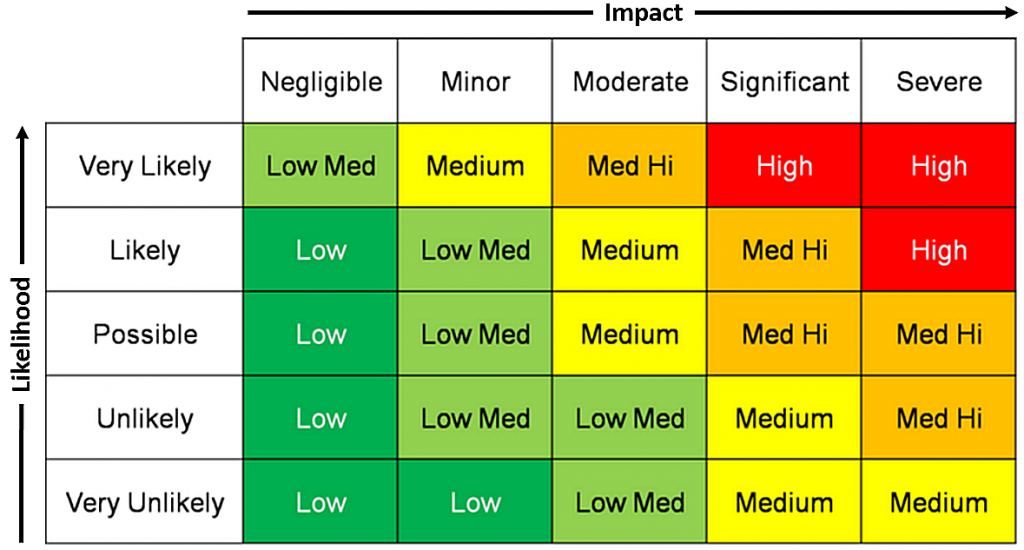
\includegraphics[width=\textwidth]{risk_matrix.png}
  \caption[Risk matrix.]{Risk matrix. From \url{https://www.armsreliability.com/page/resources/blog/beyond-the-risk-matrix}.}
  \label{fig:risk_matrix}
\end{figure}


\section{Physical Health}
In a standard office, work is often long, repetitive, and stationary. Bad posture, uncomfortable chairs, mispositioned monitors, wrist strain over cramped keyboards, poor lighting or glare are just a few of the most common risks and hazards to physical health. 

At Accenture and home, the following precautions were observed:
\begin{enumerate}
  \item Education on the proper position to work in was studied from \ref{fig:posture_desk}. Notably, the height of the chair is set to the appropriate height to allow feet to rest in an almost \SI{90}{\deg} angle, the top of the monitor edge at eye level, and the monitor slightly tilted up to equalise the distance to all corners of the screen. 
  \item Good chairs were selected. I purchased a Herman Miller Aeron chair for work at home, known for its world-renowned ergonomics. 
  \item Used a second external monitor to relieve neck strain, as it is possible to adjust the monitor's position to the optimal position. This also provided a significant productivity boost. The brightness was also adequately adjusted to bring the most comfort to the eyes. 
  \item A standing desk was purchased for working at home. 
  \item Regular breaks were taken with the team during the time at the office. 
  \item An ergonomic keyboard, the Kinesis Advantage 2, was used to relieve wrist strain and improve productivity with the features such as macros. 
\end{enumerate}

\begin{figure}[H]
  \centering
  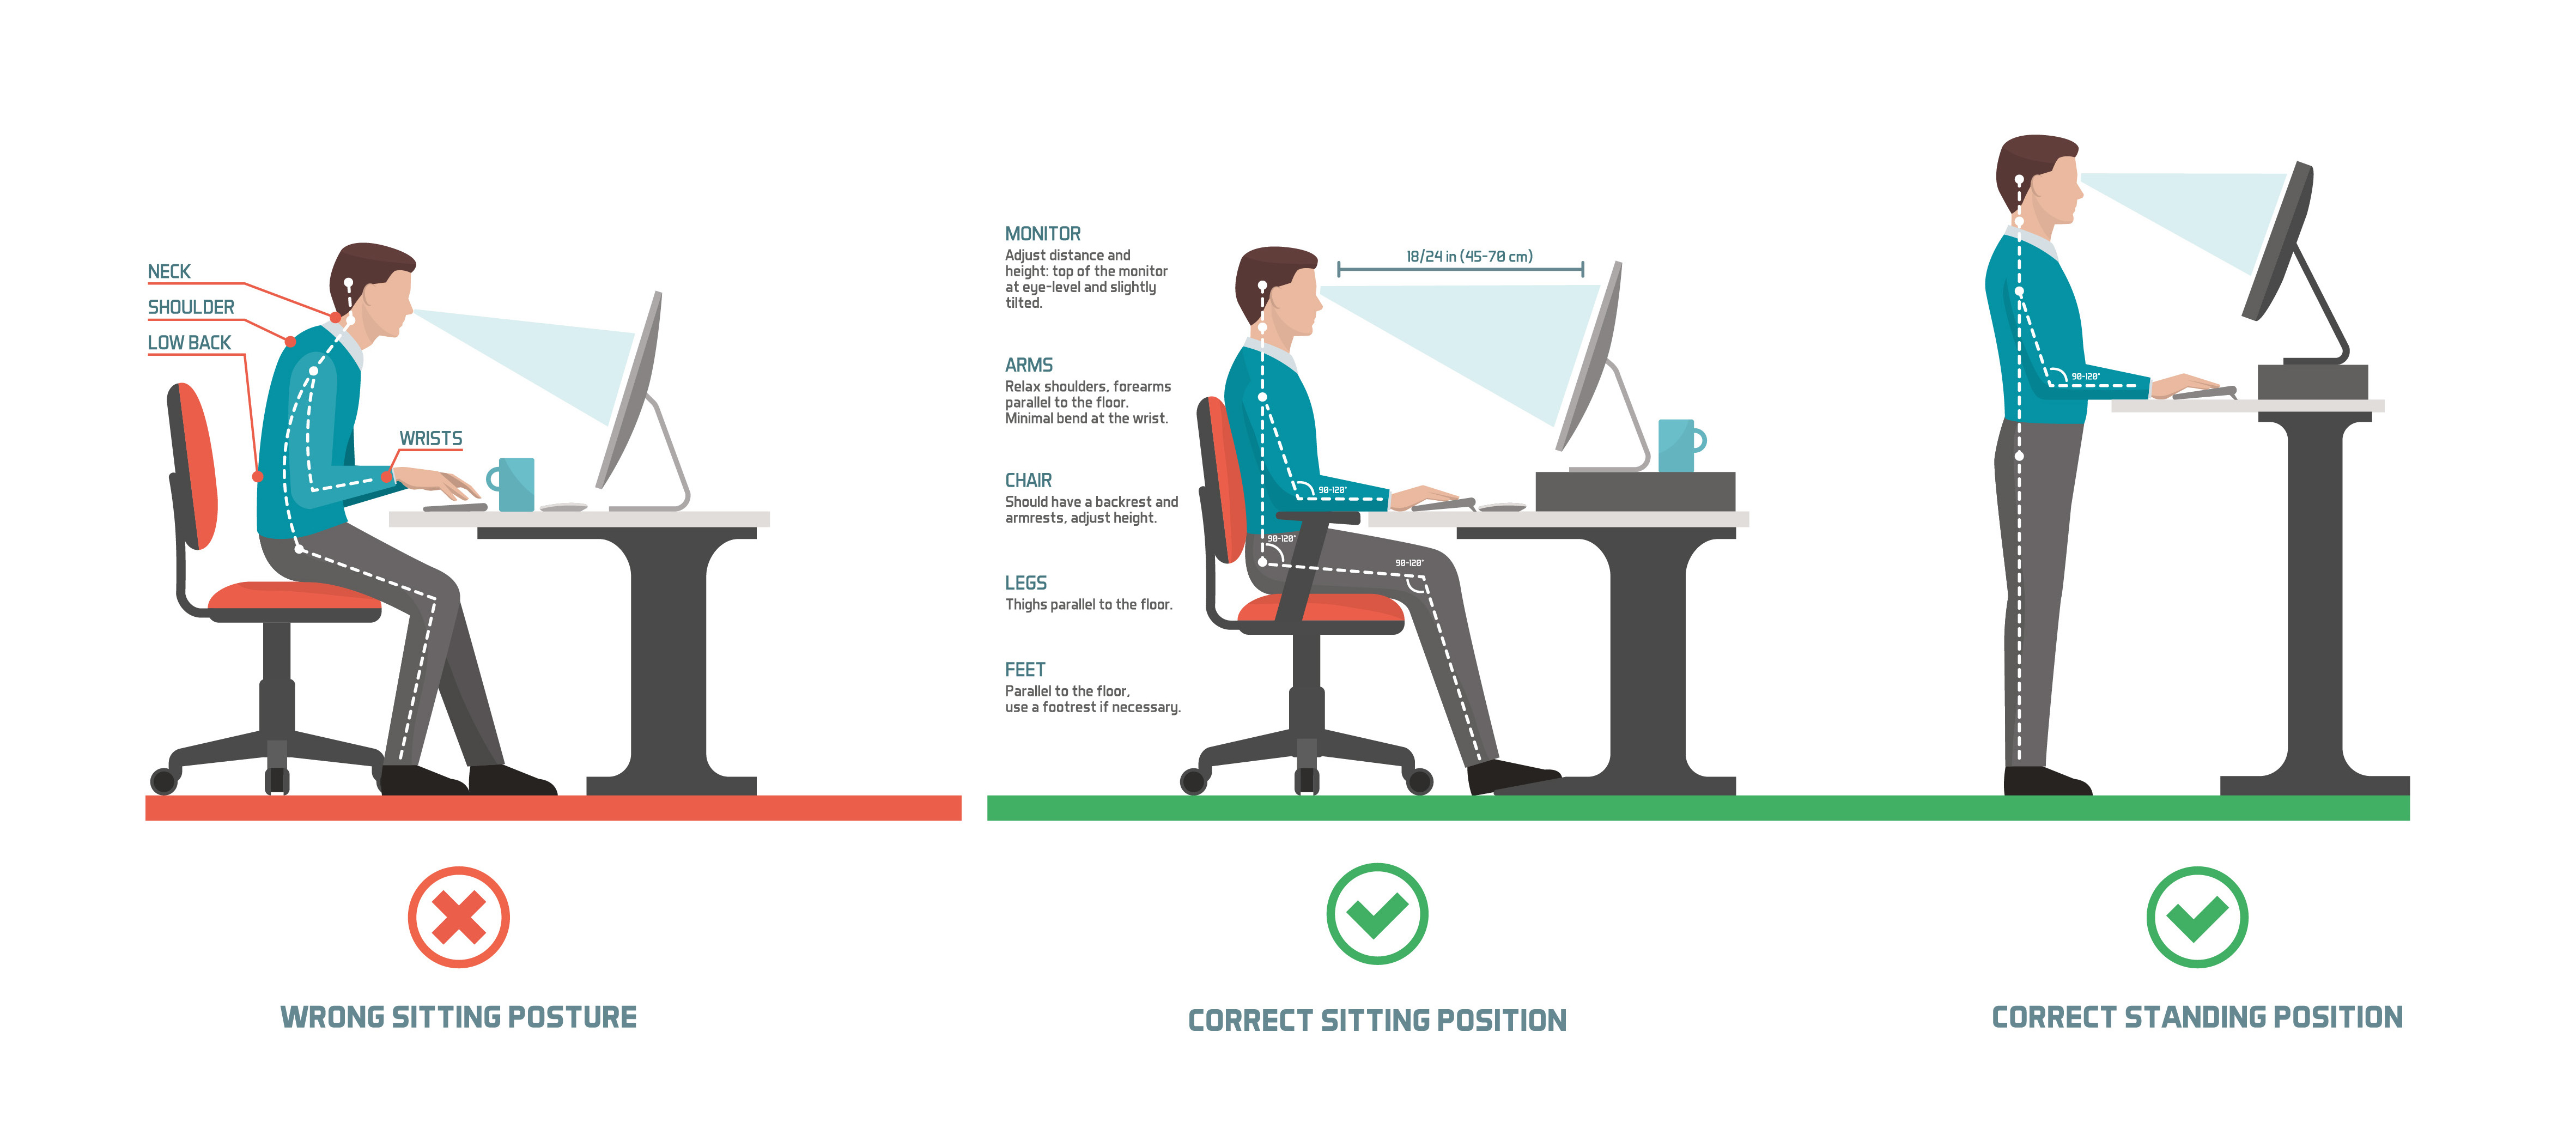
\includegraphics[width=\textwidth]{posture_desk.jpeg}
  \caption[Best posture at a desk.]{Best posture at a desk. From: \url{https://healthandbalance.com.au/workstation-desk-posture-ergonomics/}}
  \label{fig:posture_desk}
\end{figure}

Although there are many sources of long-term physical issues, these can be easily managed with awareness and mitigated effectively, resulting in a low level of risk. 

\section{Covid-19 precautions}
Covid-19 has undeniably impacted the world in many ways. This highly infectious disease caused major lockdowns and shifted work from the office to the home for extended periods. In order to follow national and state requirements, Accenture and employees worked remotely and suspended office visits. Return to the office was first announced in mid-November, where a number of precautions were followed:

\begin{enumerate}
  \item All state and national requirements were followed, including masks in public indoor areas and on transport, QR code check-ins in all locations required, and mandatory bookings for visits to the office.
  \item Social distancing in all public areas. 
  \item Sanitising hands on every entry to the office.
  \item Disallowing guest visits to the office. 
\end{enumerate}

Although the severity of symptoms one suffers from contracting Covid-19 vary wildly in the younger age group, the potential to be sick for a week or more, in addition to the mandatory self-isolation period, is highly disruptive to work and the greater population. As such, the threat of Covid-19 results in high risk. 


\section{Mental health}
Mental health is an often under-looked part of one's health. It varies greatly from person to person, and many factors play into one's overall mental health, including social health, work-life balance, and financial status. Without careful consideration, planning and awareness of one's mental health, the employee's productivity may drop sharply. 

A number of precautions were taken to care for my mental health:
\begin{enumerate}
  \item Ensuring I was enjoying the work I was doing. I transferred internally between teams to find more exciting work that I could grow and learn in while also finding a more relevant thesis topic aligned with my interests. 
  \item Coming into the office when practical. Although there were many days where I was the only team member in the office, being able to experience the office, grab hot drinks in the morning with colleagues, and work in an environment separate from home was very beneficial.
  \item Preventing work hours from extending into my personal time too often. 
\end{enumerate}

Mental health is a complex risk to quantify since it is difficult to measure and includes many factors. Overall the onus is mainly on the employee to ensure they take the proper precautions and use the available resources such as sick leave or personal time off. Particularly with the challenging program that is ESIPS, this risk is categorised as a moderate risk. 


	% Can be deleted if not a SIPS thesis
	\ifSipsThesis
% 		%!TEX root = ../thesis.tex
%!TeX spellcheck = en_GB 
% ******************** SIPS Practical Experience Reporting ********************

\chapter{Practical Experience Overview}
\label{app:prac_ex_overview}










	\fi
\end{appendices}

% *************************************** Index ********************************
\printthesisindex % If index is present

\end{document}
